\documentclass{aastex62}

\newcommand{\vdag}{(v)^\dagger}
\newcommand\aastex{AAS\TeX}
\newcommand\latex{La\TeX}

\graphicspath{{./}{figures/}}

\accepted{March 24, 2020}

\shorttitle{M33 Stellar Streams}
\shortauthors{Webster}

\begin{document}

\title{Sweet Streams are Made of This: M33 Stellar Streams During and After MW/M31 Merger.}

\author{Ryan Webster}
\email{ryanwebster@email.arizona.edu}
\affiliation{University of Arizona, Department of Astronomy}

\section{Introduction} \label{sec:intro}

The collision and merger event between the Milky Way (MW) and Andromeda Galaxy (M31) is expected to begin four and a half billion years from now. During this event, the Local Group's (LG) third largest companion, the Triangulum Galaxy (M33), will most likely orbit around the larger two galaxies during and after the merger, with only a 7{\%} chance of being ejected from the LG \cite{van_der_Marel_2012}. Over the course of the merger, tidal forces from MW and M31 are expected to strip stars, gas and dust from M33, creating tidal stellar streams. My research project aims to evaluate the morphology and evolution of M33's stellar streams over the course of the MW/M31 merger. 

With the help of large sky surveys like the Sloan Digital Sky Survey and Gaia, several examples of stellar streams have been found around the MW \cite{article}. Their progenitors are commonly found along the length of the stream and are typically dwarf galaxies or globular clusters, which orbit the MW. The streams themselves originate as the satellites being to fall into, or near, their host galaxy where tidal forces between the two bodies strip the satellite of its stellar material. These striped stars create filament structures which lead and trail the satellite as it orbits around its host galaxy. Other surveys, like those conducted by \cite{Mart_nez_Delgado_2010} reveal stellar streams around other galaxies in our local universe. This indicates that satellite in-falls are not exclusive to the MW, and are a common evolutionary characteristic for many, if not all, spiral galaxies in the universe.

The literature discussing stellar streams coinciding with an on-going galaxy merger is sparse, as most research focuses on a simple galaxy surrounded by a satellite. However, I believe these studies will still provide an appropriate starting point for my analysis. In particular, several studies using N-body simulations of galaxies with satellite in-falls have explored how the morphology of the resulting streams is effected overtime by gravitational influences from the two bodies. A study from \cite{10.1093/mnras/stw2229} found a relationship between the kinematics of stars contributed by a satellite and the mass of the satellite. Stars from more massive satellites have lower velocity dispersion, and lose angular momentum to dynamical friction. On the other hand, smaller satellites contribute fast moving stellar systems. 

N-body simulations from \cite{10.1111/j.1365-2966.2007.12313.x} investigated the dynamics responsible for creating tails from dwarf galaxy interactions. In particular, they found that ``the points where the attractive force of host halo and satellite are balanced do not occur at equal distances from the satellite centre or at the same equipotential value for massive satellites, breaking the morphological symmetry of the leading and trailing tails'' (Abstract). They also found that the satellite's gravity accelerates the trailing filament, and decelerates the leading filament, creating differences between ejecta and satellite orbits. This is seen in Figure 17 of the paper, attached below. This also means the leading tail is located well inside satellite's orbit, while the trailing tail is well outside the orbit. These are valuable insights for predicting what M33's stellar streams will look like in the simulation.

Given that many studies focus on the galaxy/satellite pairs that are not undergoing a merger, my analysis of M33's streams will incorporate new dynamics not previously explored. Comparisons between the findings of these studies and my analysis will provide insight into the complexity of stellar streams in exotic environments. It will address the effect that two large gravitational bodies have on the evolution of a smaller system's stellar streams.

\begin{figure}[htp]
    \centering
    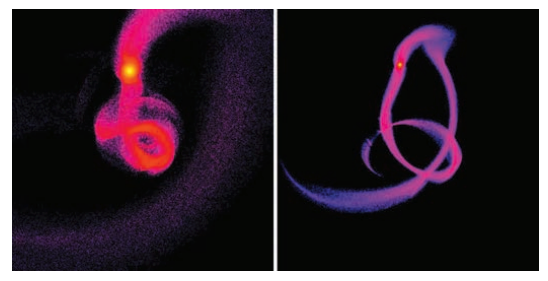
\includegraphics[width=9cm]{choi_fig17.png}
    \caption{Figure 17 from \cite{10.1111/j.1365-2966.2007.12313.x} showing in-fall simulation of a massive satellite (left) and lower mass satellite (right). The symmetry of the leading and trailing tails is clearly broken.}
    \label{fig:galaxy}
\end{figure}

\section{Proposal} \label{sec:Proposal}

My project will be addressing 3 main questions concerning the kinematics, morphology and evolution of M33's stellar streams. 

\begin{enumerate}
    \item I will look at the stream's velocity gradients and velocity dispersion, and how they will change in the MW/M31 potential. Several of the findings from \cite{10.1093/mnras/stw2229} will be of use for this analysis. Assuming M33 falls into the massive satellite regime of the \cite{10.1093/mnras/stw2229} simulation, I will investigate the low velocity dispersion and loss of angular momentum predicted in his simulations. This should be apparent in the radial velocity dispersion of M33 as it orbits the merging galaxies. \cite{10.1093/mnras/stw2229} suggests a radially biased stellar population, which is characterized by a high radial velocity, is caused by a massive satellite in-fall. 
    \item The degree to which streams trace the orbit of the satellite galaxy is explored heavily in \cite{10.1111/j.1365-2966.2007.12313.x} As discussed previously, the shape of the stream's leading and trailing tails are influenced by the satellite's self gravity. These effects should be visible in the merger simulation.
    \item The formation of stellar streams is dependent on the tidal forces between the satellite and its host, which means its influenced by the host's gravitational potential well. The potential well between MW and M31 will evolve over the course of the simulation, getting deeper as the two galaxies merge. I aim to analyze when and how M33's streams begin to form around this evolving system, and compare this evolution to other N-body simulations.
\end{enumerate}

To answer these questions, I will mostly use M33's data from the merger simulation. I plan on using multiple snapshots over the course of the merger to see how M33 changes over time. I can use the OrbitCOM.py script to track M33's center of mass as it revolves around the other two galaxies. I plan on writing a script to calculate the velocity dispersion and velocity gradient of M33 at each snapshot. I will also attempt a visualization of the orbit along with the leading and trailing tails of M33 to investigate how well they correlate, as in Figure 8 from \cite{10.1111/j.1365-2966.2007.12313.x}.

My prediction is the streams will not closely follow the orbit of M33. The evidence for a morphological asymmetry during satellite in-falls, especially for massive systems, is strong from \cite{10.1111/j.1365-2966.2007.12313.x}. I also predict that the added dynamics of a MW M31 merger will complicate the dynamics of the stellar streams, making many of the predictions from \cite{10.1093/mnras/stw2229} difficult to observe.

\begin{figure}[htp]
    \centering
    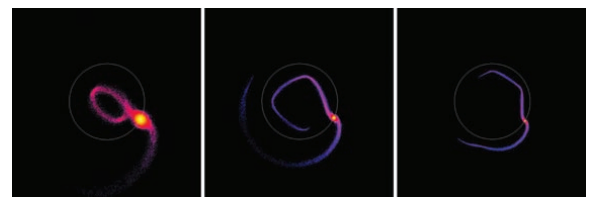
\includegraphics[width=13cm]{choi_fig8.png}
    \caption{Figure 8 from \cite{10.1111/j.1365-2966.2007.12313.x} showing streams plotted against the orbit of the satellite. From left to right, the panels are for massive, low-mass and tiny-mass satellites. I expect M33 to exhibit the behavior of the massive system.}
    \label{fig:galaxy}
\end{figure}

\bibliography{references}{}
\bibliographystyle{aasjournal}

\end{document}
